\chapter{Estado da Arte} \label{chap:sota}

\section{Arquiteturas de Redes UAV}

Dependendo do contexto em que estão inseridos, os UAVs podem estar dispostos de diversas formas e podem também ser controlados de diferentes formas. Ao longo desta secção serão analisadas diferentes arquiteturas de redes UAV o modo como funcionam e como interagem os UAVs entre si e em rede.

\subsection{Controlo Directo}
Neste tipo de arquitetura cada UAV é controlado diretamente pela sua estação controladora, fazendo com que não exista qualquer tipo de interação inter-UAV. Sendo que cada comando é enviado diretamente para cada UAV e sendo executado apenas pelo próprio como demonstrado na figura \ref{fig:controlo_directo}.

\begin{figure}[H]
\centering
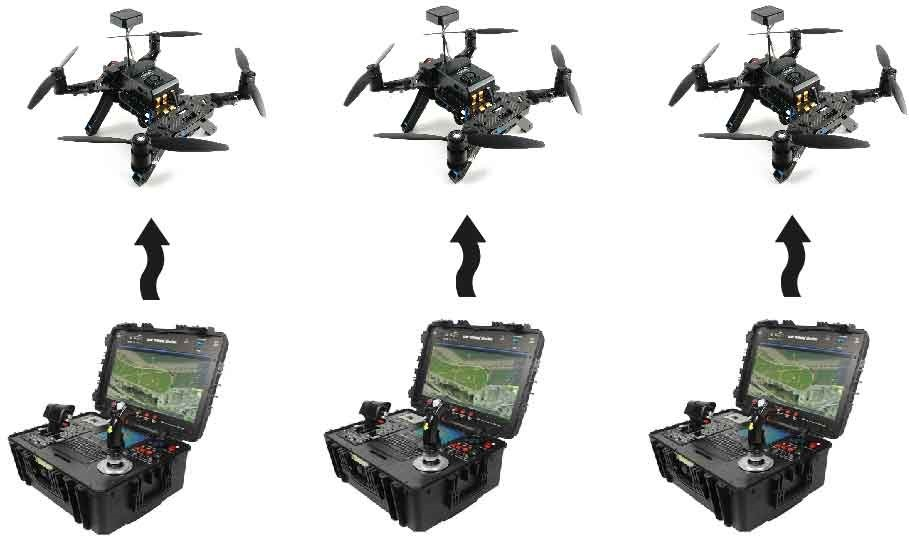
\includegraphics[width=60mm]{controlo_direto}
\caption{A arquitectura de controlo directo \label{fig:controlo_directo}}
\end{figure}

As GCSs podem ser implementadas de diferentes formas, podem ser implementadas através de uma antena Wi-Fi, que distribui o sinal de comando para os UAVs. Ou então, numa versão mais simples através de telecomando sendo que esta é opção a mais utilizada em captação de imagem e vídeo.

No entanto, como esta arquitectura é baseada num modelo de controlo mais centralizado possui algumas desvantagens tais como: 

\begin{itemize}
\item Se houver um ponto de falha, o sistema fica comprometido;
\item Nem todos os UAVs estão ligados à GCS a todo o instante, e assim os sinais de controlo podem não chegar ao drone;
\item E por fim, pode constituir um problema não só para comunicação mas também, para a segurança do sistema \cite{ImadJawhar2017}.
\end{itemize}

\subsection{Enxames de UAVs}

Um enxame de UAVs é capaz de formar redes expansíveis, para além das infraestruturas, que permitem o acesso dos nós terrestres. Ao beneficiar dos recursos de alta flexibilidade e de rápida provisão, a \textit{swarm} de UAVs é uma solução viável para recuperar a comunicação de forma rápida e eficaz, especialmente para cenários onde os recursos de comunicação são escassos ou inexistentes, como nos ambientes pós-desastre \cite{Shi2018}. 

Nesta arquitetura, as ligações d2d, \textit{drone-to-drone} são necessárias para fazer a comunicação entre os UAVs existentes no enxame. Num enxame de UAVs, existe uma hierarquia que é constituída por um líder e pelos seguidores. O líder é o UAV que recebe os comandos, e os seguidores são os que seguem a rota do líder e os comandos que lhe são passados por este.

\begin{figure}[H]
\centering
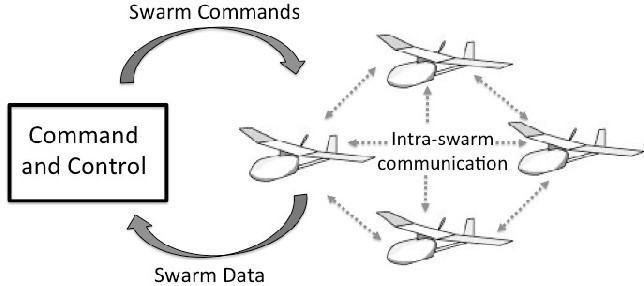
\includegraphics[width=10cm]{uav_swarm}
\caption{Diagrama de Controlo e Comando de um enxame UAV\label{fig:uav_swarm} }\cite{G.Madey2013}
\end{figure}

Esta topologia suporta não só a troca de mensagens de controlo entre os UAVs, de modo a prevenir colisões e a calcular rotas de voo,  bem como a transmissão dos dados para serem acedidos por outros UAVs. Existem UAVs específicos dentro do enxame que estão equipados com interfaces para comunicar com as infraestruturas ou satélites, estes estabelecem as \textit{gateways} entre o enxame e as outras redes.

Nos meios rurais ou em meios de pós-desastre onde as infraestruturas de cobertura são escassas, os enxames UAV são formados como infraestruturas aéreas temporárias para os veículos \cite{Shi2018}.

No exemplo citado no artigo \cite{He2018}, é estudada a possibilidade de um enxame de UAVs através do algoritmo proposto contar com vários líderes e também ao longo do tempo haver a possibilidade de aumentar o número de seguidores, a fim de reduzir o consumo de comunicação e melhorar a adaptabilidade do sistema e também a sua expansibilidade.

\subsection{Redes Mesh}

A rede \textit{mesh} sem fio consiste em nós de rádio organizados em uma topologia \textit{mesh} ou malha. São normalmente compostas por \textit{routers} e \textit{gateways mesh} que distribuem o sinal de \textit{Wi-Fi} igualmente por todos os pontos da rede.

Nestes cenários de rede, os \textit{routers} comunicam entre si e enviam sinal \textit{Wi-Fi} reciprocamente, bem como, para a área envolvente. Por exemplo, se um nó A quiser comunicar com o nó C irá utilizar o nó B que fica entre ambos para fornecer melhor possibilidade de comunicação. 

A este nó B, que se refere a um ponto intermediário, dá-se o nome de “salto” ou “\textit{hops}” da rede mesh. Cada um destes saltos, introduz um nível de atraso na rede, por isso é necessário que o número de saltos seja minimizado encontrando por exemplo o caminho mais direto entre os dois nós. No entanto, quando um dos \textit{routers} da rede \textit{mesh} fica \textit{offline} ou inutilizado o sinal consegue encontrar outros caminhos graças aos nós alternativos \cite{NetSpot}.

Nesta configuração de rede mesh encontra-se o projeto UAVNet referenciado pelo artigo \cite{Morgenthaler2012a}, que é uma \textit{framework} baseada numa altamente adaptável \textit{wireless mesh network}, WMN, que faz uso de UAVs pequenos equipados com \textit{wireless mesh nodes}, conectados aos UAV via porta série, de modo a poder interagir como uma \textit{mesh} em pleno ar.

\begin{figure}[H]
\centering
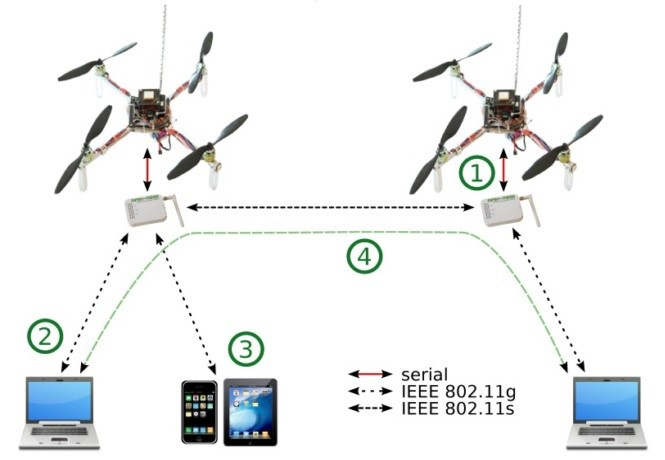
\includegraphics[width=10cm]{uav_net}
\caption{Exemplo de aplicação do \textit{UAVNet} \label{fig:uav_net} }\cite{Morgenthaler2012a}
\end{figure}

\subsection{Redes Ad-Hoc}

A tecnologia \textit{ad-hoc} permite a criação de redes de dispositivos móveis em áreas onde não existem infraestruturas de comunicações. Neste tipo de ligação não existe um nó central para onde todas as informações são enviadas pelos outros nós, fazendo com que não seja necessária a existência de um \textit{router} que faça a comunicação da rede com outros dispositivos externos. As ligações entre nós são independentes entre si, de maneira que, se uma falhar, seja por perda de conexão ou falha de algum dispositivo, todas as outras ligações continuam a funcionar \cite{DalloraMoraes2007}.

Como as redes \textit{ad-hoc} funcionam sem nenhuma infraestrutura é necessário que existam mecanismos de descoberta de rotas e encaminhamento de informação para isso estas redes recorrem a protocolos de rotas de dois tipos: os reativos e os pró-ativos.

Dentro dos protocolos reativos, que são protocolos que não tomam iniciativa de manter as rotas e apenas as determinam quando necessário fazendo \textit{flooding} de pedidos na rede. Este protocolo tem como vantagem o facto de usar recursos apenas quando é necessário, no entanto, inundam a rede com pedidos e introduzem atraso no inicio de envio do tráfego pois tem de ser primeiramente determinada a rota. Neste tipo de protocolos inclui-se o AODV definido pela norma RFC 3561, onde um determinado nó A envia um \textit{Route Request} para poder efetuar a comunicação com o nó B e recebe deste um \textit{Route Reply} de forma a indicar a rota mais próxima.

No caso dos protocolos pró-ativos, as rotas são construídas utilizando tráfego de controlo contínuo e mantém todas as rotas. Este processo tem como vantagem ter as rotas sempre disponíveis e mantém o tráfego de controlo constante. Um exemplo deste tipo de protocolo é o OLSR definido pela norma RFC 3626. Este protocolo implementa um sistema de deteção de ligação a nós vizinhos, através de mensagens \textit{HELLO}, efetua os pedidos de encaminhamento de forma otimizada através do mecanismo de MPR. Para além destes dois aspetos este protocolo envia mensagens de estado das ligações e cálculo de rotas \cite{Ricardoa}.

Em relação aos drones existem já estudos sobre as FANETs, que são redes \textit{ad-hoc} constituídas por UAVs, como se pode comprovar através do artigo \cite{Bekmezci2013a}. Um dos exemplos de rede ad-hoc com equipamentos UAV é o que está referenciado no artigo \cite{Brown2004} que fala de dois cenários de funcionamento, no primeiro o UAV atua como um nó de rádio  a proeminente que efetua a conexão de dos pontos de rádio terrestres desativados. No segundo cenário, a rede permite que os grupos de UAVs comuniquem entre si para estender o alcance operacional dos UAVs mais pequenos.

\begin{figure}[H]
\centering
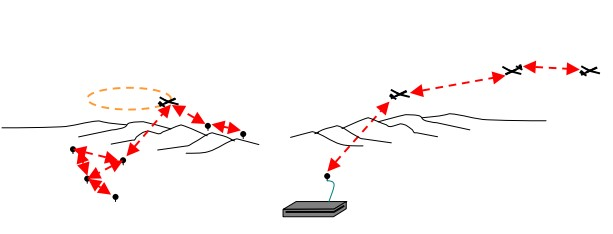
\includegraphics[width=10cm]{ad-hoc_protocols}
\caption{Figuras ilustrativas do cenário 1 (esquerda) e do cenário 2 (direita)  \label{fig:ad-hoc_protocols}}
\cite{Ricardoa}
\end{figure}

\subsection{Redes SD-UAV}

As redes definidas por software (SDN) são o novo paradigma de \textit{networking} no qual o \textit{hardware} de encaminhamento é dissociado das decisões de controlo. É uma tecnologia que promete simplificar a gestão da rede e permitir a inovação e evolução. A ideia principal é permitir que os software developers confiem nos recursos de rede da mesma maneira que fazem com os recursos de armazenamento e computação. Nas SDN, a inteligência da rede é centralizada logicamente nos controladores baseados em \textit{software} (plano de controlo) e os dispositivos de rede tornam-se simples dispositivos de encaminhamento de pacotes (plano de dados) que podem ser programados através de uma interface aberta \cite{Nunes2014} (ex. OpenFlow \cite{Leon-Garcia2015}, etc).

No artigo \cite{Secinti2018} é proposto um protocolo de gestão de uma rede aérea contruído em cima de uma arquitetura SDN. Neste projeto cada UAV torna-se num switch SDN que é controlado por diretivas enviadas por um controlador centralizado.

\begin{figure}[H]
\centering
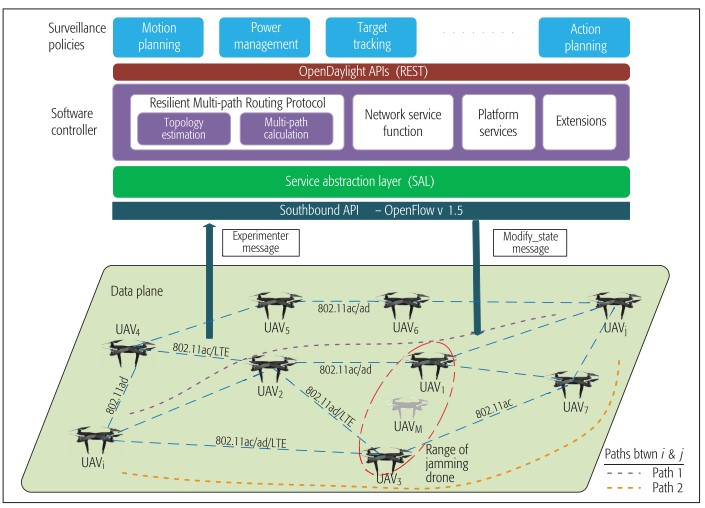
\includegraphics[width=10cm]{sd-uav_architecture}
\caption{Arquitetura SD-UAV proposta no artigo  \label{fig:sd-uav_architecture} }\cite{Secinti2018}
\end{figure}



\section{Áreas de aplicação das redes UAV}

\subsection{Retransmissão de Comunicação}
\subsection{Gateways de Rede}
\subsection{UAV-assisted Sensing}
\subsection{UAV-assisted Acting}
\subsection{UAV-based data storage}
\subsection{UAV-based data processing}


\section{Software de Controlo Open-Source}

\subsection{Papparazzi UAV}
\subsection{ArduPilot}
\subsection{Dronecode}
\subsection{LibrePilot}
\subsection{Comparação de soluções}



